\subsection{Passenger Reservation}
\subsubsection{Scenario}
It is 9.00 in the morning and Tom has already downloaded the mobile application called \textit{myTaxiService} and he has a fixed appointment at 17.00 at "Stazione Centrale of Milano" so he decides to reserve a taxi for the 16.30 to go there. He enters in the apposite section of the application, indicates the source of the journey,the destination, the time of the meeting with the Taxi driver. He also specify the number of passengers that the Taxi will carry. The system, after a few seconds, reply positively to Tom saying that the reservation has been accepted and that the Taxi identification number will be provided 10 minutes before the meeting time.

\subsubsection{Use case}
\begin{center}
	\begin{longtable}{| p{.20\textwidth} | p{.80\textwidth} |} \hline
		Use case & \textbf{Reserve a taxi} \\ \hline 
		Actors & Passenger, Taxi Driver \\ \hline
		Goals & A passenger must be able to reserve a taxi ride from an origin, to a destination at a specific time and date \\ \hline
		Enter condition & \begin{itemize}
			\item The Passenger must already be registered to the service
			\item The Taxi driver must be registered to the service
			\item The Passenger must already have opened the application (mobile or web) and logged in
			\item The Taxi driver must be available to accept requests
		\end{itemize} \\ \hline
		Event flow & \begin{enumerate}
			\item The Passenger goes to the section for reserving a taxi ride
			\item \label{fillForm} The Passenger fills the form with:
			\begin{itemize}
				\item Origin
				\item Location
				\item Date
				\item Time
				\item Number of passengers
			\end{itemize}
			\item The Passenger submit the request to the system
			\item If there are errors with the data (missing fields, not valid locations or number of passengers greater than 3) or the date and time provided are not 2 hours in advance:
			\begin{enumerate}
				\item The system notifies the error to the Passenger
				\item Go back to Event flow \ref{fillForm}
			\end{enumerate}
			\item The reservation is stored in the system
			\item The system waits until 10 minutes before the date and time of the reservation
			\item The system checks the origin location provided by the Passenger and computes the corresponding zone in the city
			\item The system, based on the city zone computed, retrieves the corresponding taxi queue
			\item If there are no taxi in the queue: \label{noTaxi}
			\begin{enumerate}
				\item Returns an error to the Passenger and invites him to make a request
				\item Go back to Event flow \ref{fillForm}
			\end{enumerate}
			\item The system takes the first taxi in the queue
			\item The system send the request to the taxi driver
			\item If the taxi driver does not accept the request:
			\begin{enumerate}
				\item The system puts the Taxi driver at the bottom of the queue
				\item Go back to Event flow \ref{noTaxi}
			\end{enumerate}
			\item The system sends to the Taxi driver the location of the meeting point with the Passenger
			\item The system computes an approximate waiting time for the Passenger
			\item The system informs the Passenger of the forthcoming arrival of the Taxi and the approximate waiting time.
		\end{enumerate} \\ \hline
		Exceptions & The passenger can abort the procedure only during the	waiting phase. If he decides to abort the procedure:
		\begin{enumerate}
		\item If the time of cancellation of the reservation is later than 10 minutes before the meeting time:
		\begin{enumerate}
			\item The system notifies the Passenger of the impossibility to cancel the reservation
		\end{enumerate}
		\item The system cancel the reservation
		\item The system notifies the Passenger of the successful deleting of the reservation
		\end{enumerate} \\ \hline
Exit condition & The passenger is waiting for the taxi driver and a Taxi driver is reaching him
		\\ \hline
		\caption{Use case: Taxi reservation from a passenger}+
		\label{reserveTaxiUC}
	\end{longtable}
\end{center}

\subsubsection{Sequence diagram}
\begin{figure}[H]
\centering
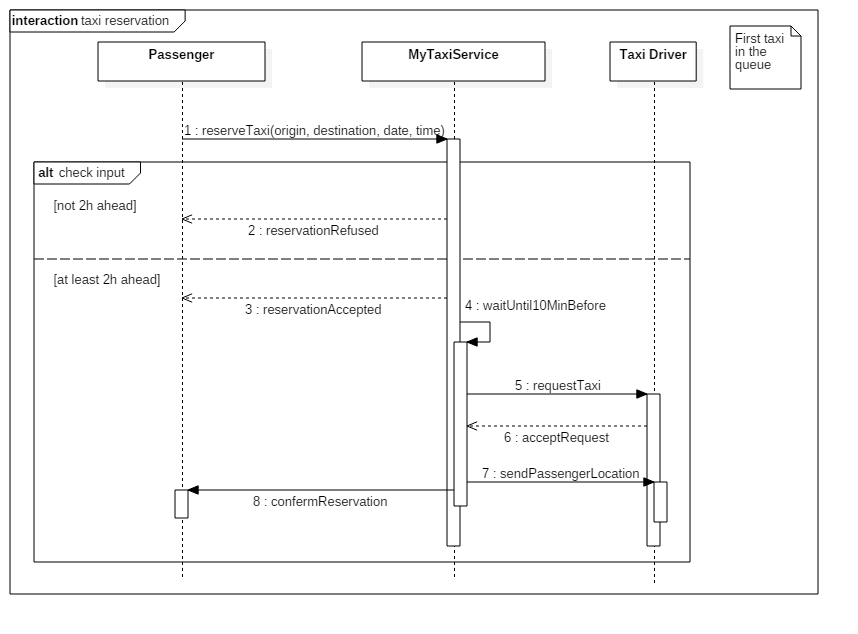
\includegraphics[scale=0.5]{Images/sequence_taxi_reservation}
\caption{Reservation of a taxi}
\label{reserve_taxi_SD}
\end{figure}



